\documentclass{article}

\usepackage{fancyhdr}
\usepackage{extramarks}
\usepackage{amsmath}
\usepackage{amsthm}
\usepackage{amsfonts}
\usepackage{tikz}
\usepackage[plain]{algorithm}
\usepackage{algpseudocode}

% \usepackage{bbold}
\usepackage{dsfont}
\usepackage{braket}
\usepackage{cancel}
\usepackage{booktabs}
\usepackage{graphicx}

\usetikzlibrary{automata,positioning}

%
% Basic Document Settings
%

\topmargin=-0.45in
\evensidemargin=0in
\oddsidemargin=0in
\textwidth=6.5in
\textheight=9.0in
\headsep=0.25in

\linespread{1.1}

\pagestyle{fancy}
\lhead{\hmwkAuthorName}
\chead{\hmwkClass: \hmwkTitle}
\rhead{\firstxmark}
\lfoot{\lastxmark}
\cfoot{\thepage}

\renewcommand\headrulewidth{0.4pt}
\renewcommand\footrulewidth{0.4pt}

\setlength\parindent{0pt}

%
% Create Problem Sections
%

\newcommand{\enterProblemHeader}[1]{
    \nobreak\extramarks{Problema \arabic{#1}}{}
}

\newcommand{\exitProblemHeader}[1]{
    \nobreak\extramarks{Problema \arabic{#1}}{Problema \arabic{#1}}
    \stepcounter{#1}
    \nobreak\extramarks{Problema \arabic{#1}}{}
}

\setcounter{secnumdepth}{0}
\newcounter{partCounter}
\newcounter{homeworkProblemCounter}
\setcounter{homeworkProblemCounter}{1}
\nobreak\extramarks{Problema \arabic{homeworkProblemCounter}}{}\nobreak{}

%
% Homework Problem Environment
%
% This environment takes an optional argument. When given, it will adjust the
% problem counter. This is useful for when the problems given for your
% assignment aren't sequential. See the last 3 problems of this template for an
% example.
%
\newenvironment{homeworkProblem}[1][-1]{
    \ifnum#1>0
        \setcounter{homeworkProblemCounter}{#1}
    \fi
    \section{Problema \arabic{homeworkProblemCounter}}
    \setcounter{partCounter}{1}
    \enterProblemHeader{homeworkProblemCounter}
}{
    \exitProblemHeader{homeworkProblemCounter}
}

%
% Homework Details
%   - Title
%   - Due date
%   - Class
%   - Section/Time
%   - Instructor
%   - Author
%

\newcommand{\hmwkTitle}{Compiti \#3}
\newcommand{\hmwkDueDate}{14 Nov, 2022}
\newcommand{\hmwkClass}{Fisica Teorica della Materia}
% \newcommand{\hmwkClassTime}{Section A}
% \newcommand{\hmwkClassInstructor}{Professor Isaac Newton}
\newcommand{\hmwkAuthorName}{\textbf{Gianluca Zappavigna}}

%
% Title Page
%

% \title{
%     \vspace{2in}
%     \textmd{\textbf{\hmwkClass:\ \hmwkTitle}}\\
%     \normalsize\vspace{0.1in}\small{Due\ on\ \hmwkDueDate\ at 3:10pm}\\
%     \vspace{0.1in}\large{\textit{\hmwkClassInstructor\ \hmwkClassTime}}
%     \vspace{3in}
% }

% \author{\hmwkAuthorName}
% \date{}

\renewcommand{\part}[1]{\textbf{Parte \arabic{partCounter}}\stepcounter{partCounter}\\}

%
% Various Helper Commands
%

% Useful for algorithms
\newcommand{\alg}[1]{\textsc{\bfseries \footnotesize #1}}

% For derivatives
\newcommand{\deriv}[1]{\frac{\mathrm{d}}{\mathrm{d}x} (#1)}

% For partial derivatives
\newcommand{\pderiv}[2]{\frac{\partial}{\partial #1} #2}

% Integral dx
\newcommand{\dx}{\mathrm{d}x}

% Alias for the Solution section header
\newcommand{\solution}{\textbf{\large Solution}}

% Probability commands: Expectation, Variance, Covariance, Bias
\newcommand{\E}{\mathrm{E}}
\newcommand{\Var}{\mathrm{Var}}
\newcommand{\Cov}{\mathrm{Cov}}
\newcommand{\Bias}{\mathrm{Bias}}

\begin{document}
% \maketitle
% \pagebreak

\begin{homeworkProblem}
    \part

    Per bosoni, due o più particelle possono trovarsi nello stesso stato energetico.

    \begin{table}[h]
        \begin{center}
            \footnotesize%
            \begin{tabular}{llcccr}
            \toprule
            E & stato (degenerazione) & degenerazione complessiva ($g$) \\
            \midrule
            $0$ & $\Ket{0, 0, 0}$ $\left(1\right)$ & 1 \\
            $\varepsilon$ & $\Ket{\varepsilon, 0, 0}$ $\left(\binom{3}{1} = 3\right)$ & 3 \\
            $2\varepsilon$ & $\Ket{\varepsilon, \varepsilon, 0}$ $\left(\binom{3}{2} = 3\right)$, $\Ket{2\varepsilon, 0, 0}$ $\left(\binom{3}{1} = 3\right)$  & 6 \\
            $3\varepsilon$ & $\Ket{2\varepsilon, \varepsilon, 0}$ $\left(3! = 6\right)$, $\Ket{\varepsilon, \varepsilon, \varepsilon}$ $\left(1\right)$  & 7 \\
            $4\varepsilon$ & $\Ket{2\varepsilon, 2\varepsilon, 0}$ $\left(\binom{3}{2} = 3\right)$, $\Ket{2\varepsilon, \varepsilon, \varepsilon}$ $\left(\binom{3}{2} = 3\right)$ & 6 \\
            $5\varepsilon$ & $\Ket{2\varepsilon, 2\varepsilon, \varepsilon}$ $\left(\binom{3}{2} = 3\right)$ & 3 \\
            $6\varepsilon$ & $\Ket{2\varepsilon, 2\varepsilon, 2\varepsilon}$ $\left(1\right)$ & 1 \\
            \end{tabular}
        \end{center}
        \end{table}


    \part

    Per fermioni, le tre particelle devono tutte occupare necessariamente stati energetici diversi. Dato che ci sono solo 3
    livelli energetici, ciascuna deve trovarsi in uno di questi.

    \begin{table}[h]
        \begin{center}
            \footnotesize%
            \begin{tabular}{llcccr}
            \toprule
            E & stato (degenerazione) & degenerazione complessiva ($g$) \\
            \midrule
            $3\varepsilon$ & $\Ket{0, \varepsilon, 2\varepsilon}$ $\left(3! = 6\right)$ & 6 \\
            \end{tabular}
        \end{center}
        \end{table}

\end{homeworkProblem}

\begin{homeworkProblem}
    \part

    % \begin{equation*}
    %     x = 1
    % \end{equation*}

    Sappiamo che per l'operatore $\hat{a}^{\dagger}$ vale
    \begin{equation*}
        \hat{a}^{\dagger} \Ket{n} = \sqrt(n + 1) \Ket{n + 1}
    \end{equation*}

    Questo significa che possiamo trovare un qualunque stato $\Ket{n}$ applicando ripetutamente $\hat{a}^{\dagger}$
    \begin{equation*}
        \Ket{n} = \frac{\left(\hat{a}^\dagger\right)^n}{\sqrt{n!}} \Ket{0}
    \end{equation*}

    Il corrispondente bra risulta essere
    \begin{equation}\label{creation}
        \Bra{n} = \Bra{0} \left[\frac{\left(\hat{a}^\dagger\right)^n}{\sqrt{n!}}\right]^\dagger
        = \Bra{0} \frac{\hat{a}^n}{\sqrt{n!}}
    \end{equation}

    Attraverso la relazione di completezza possiamo scrivere $\Ket{\alpha}$ come
    \begin{equation*}
        \Ket{\alpha} = \sum_n \ket{n}\braket{n | \alpha}
    \end{equation*}

    Sfruttando \eqref{creation} troviamo
    \begin{align*}
        \Ket{\alpha} = \sum_n \ket{n}\Braket{0 | \frac{\hat{a}^n}{\sqrt{n!}} | \alpha}
        = \sum_n \ket{n}\Braket{0 | \frac{\alpha^n}{\sqrt{n!}} | \alpha}
        = \sum_n \frac{\alpha^n}{\sqrt{n!}} \ket{n}\Braket{0 | \alpha}
        = \Braket{0 | \alpha} \sum_n \frac{\alpha^n}{\sqrt{n!}} \ket{n}
    \end{align*}

    In questa espressione rimane da determinare $\Braket{0 | \alpha}$. Lo possiamo fare usando il fatto
    che $\Ket{\alpha}$ deve essere necessariamente normalizzato, cioè
    \begin{equation*}
        \Braket{\alpha | \alpha}  = 1
    \end{equation*}

    Il bra $\Bra{\alpha}$ è
    \begin{equation*}
        \Bra{\alpha }  = \Braket{0 | \alpha}^* \sum_{n'} \frac{\left(\alpha^*\right)^{n'}}{\sqrt{n'!}}\Ket{n'}
    \end{equation*}

    Ora imponendo la condizione troviamo
    \begin{gather*}
        \begin{split}
            1 = \Braket{\alpha | \alpha} = \Braket{0 | \alpha}^* \Braket{0 | \alpha} \sum_n \sum_{n'} \frac{\left(\alpha^*\right)^{n'}\alpha^n}{\sqrt{n'!}\sqrt{n!}}\Braket{n' | n} =\\
            = \left|\Braket{0 | \alpha}\right|^2 \sum_n \sum_{n'} \frac{\left(\alpha^*\right)^{n'}\alpha^n}{\sqrt{n'!}\sqrt{n!}}\delta_{n'n} = \\
            = \left|\Braket{0 | \alpha}\right|^2 \sum_n \frac{\left(\alpha^*\right)^n\alpha^n}{\sqrt{n!}\sqrt{n!}} = \\
            = \left|\Braket{0 | \alpha}\right|^2 \sum_n \frac{\left(\left|\alpha\right|^2\right)^n}{n!} = \\
            = \left|\Braket{0 | \alpha}\right|^2 \exp \left(|\alpha|^2\right) \\
        \end{split} \\
        \Longrightarrow \quad \left|\Braket{0 | \alpha}\right| = \exp \left(-\frac{|\alpha|^2}{2}\right)
    \end{gather*}

    Abbiamo determinato $\Braket{0 | \alpha}$ a meno di un segno, ma questo non è fisicamente rilevante quindi possiamo assumere che
    \begin{equation*}
        \Braket{0 | \alpha} = \exp \left(-\frac{|\alpha|^2}{2}\right)
    \end{equation*}
    e infine troviamo che

    \begin{equation*}
        \Ket{\alpha} = \exp \left(-\frac{|\alpha|^2}{2}\right) \sum_n \frac{\alpha^n}{\sqrt{n!}} \Ket{n}
    \end{equation*}
    \part

    \begin{align*}
        \Braket{0 | \alpha} = \exp \left(-\frac{|\alpha|^2}{2}\right) \sum_n \frac{\alpha^n}{\sqrt{n!}} \Braket{0 | n} = \\
        = \exp \left(-\frac{|\alpha|^2}{2}\right) \frac{\alpha^0}{\sqrt{0!}} = \exp \left(-\frac{|\alpha|^2}{2}\right) \\
        \Longrightarrow \quad \left|\Braket{0 | \alpha}\right|^2 = \exp \left(-|\alpha|^2\right)
    \end{align*}

    \part

    \begin{align*}
        \Braket{n | \alpha} = \exp \left(-\frac{|\alpha|^2}{2}\right) \sum_{n'} \frac{\alpha^{n'}}{\sqrt{n'!}} \Braket{n | n'} = \\
        = \exp \left(-\frac{|\alpha|^2}{2}\right) \frac{\alpha^{n}}{\sqrt{n!}} \\
        \Longrightarrow \quad \left|\Braket{n | \alpha}\right|^2 = \exp \left(- |\alpha|^2\right) \frac{|\alpha|^{2n}}{n!}
    \end{align*}
    \part

    \begin{align*}
        \Braket{\beta | \alpha}
        = \exp \left(-\frac{|\alpha|^2}{2}\right)\left(-\frac{|\beta|^2}{2}\right) \sum_n\sum_{n'} \frac{\left(\beta^*\right)^{n'}\alpha^n}{\sqrt{n'!}\sqrt{n!}} \Braket{n' | n} = \\
        = \exp \left(-\frac{|\alpha|^2}{2}-\frac{|\beta|^2}{2}\right) \sum_n\sum_{n'} \frac{\left(\beta^*\right)^{n'}\alpha^n}{\sqrt{n'!}\sqrt{n!}} \delta_{n' n} = \\
        = \exp \left(-\frac{|\alpha|^2}{2}-\frac{|\beta|^2}{2}\right) \sum_n \frac{\left(\beta^*\alpha\right)^n}{n!} = \\
        = \exp \left(-\frac{|\alpha|^2}{2}-\frac{|\beta|^2}{2}\right) \exp \left(\beta^*\alpha\right) = \\
        = \exp \left(-\frac{|\alpha|^2}{2}-\frac{|\beta|^2}{2} + \beta^*\alpha\right) \\
        \Longrightarrow \quad \left|\Braket{\beta | \alpha}\right|^2 = \exp \left(- |\alpha|^2 - |\beta|^2 + \beta^*\alpha + \beta\alpha^*\right) \\
    \end{align*}


\end{homeworkProblem}

\begin{homeworkProblem}
    \part

    In questo caso la dimensione dello spazio di Fock equivale a trovare il numero di possibili $M$-tuple di interi la cui somma è pari a $N$.
    Si può dimostrare che questo numero è dato da
    \begin{equation*}
        \binom{N + M - 1}{M}
    \end{equation*}

    \part

    Assumendo che $N = M$ la dimensione dello spazio di Fock diventa
    \begin{equation} \label{orig}
        \binom{N + M - 1}{M} = \binom{2N - 1}{N}
    \end{equation}

    Possiamo manipolare questa espressione, trovando
    \begin{align*}
        \binom{2N - 1}{N} = \frac{(2N - 1)!}{N!(2N-1 - N)!} = \frac{(2N - 1)!}{N!(N-1)!} =
        \frac{(2N - 1)!2N}{N!(N-1)!2N} = \frac{(2N)!}{2 N!N!} = \frac{(2N)!}{2 (N!)^2}
    \end{align*}

    Se $N \gg 1$ possiamo sfruttare l'approssimazione di Stirling e otteniamo

    \begin{align} \label{stirling}
        \frac{(2N)!}{2 (N!)^2} \simeq \frac{\sqrt{4 \pi N} \left(\frac{2N}{e}\right)^{2N}}{ 2 \cdot 2\pi N \left(\frac{N}{e}\right)^{2N}} =
        \frac{2\sqrt{ \pi N} \left(\frac{2N}{e}\right)^{2N}}{ 4\pi N \left(\frac{N}{e}\right)^{2N}} =
        \frac{\left(2N\right)^{2N}}{ 2\sqrt{\pi N} \left(N\right)^{2N}} =
        \frac{2^{2N}}{2\sqrt{ \pi N}} = \frac{2^{2N-1}}{\sqrt{ \pi N}}
    \end{align}

    \begin{figure}[h]
        \centering
        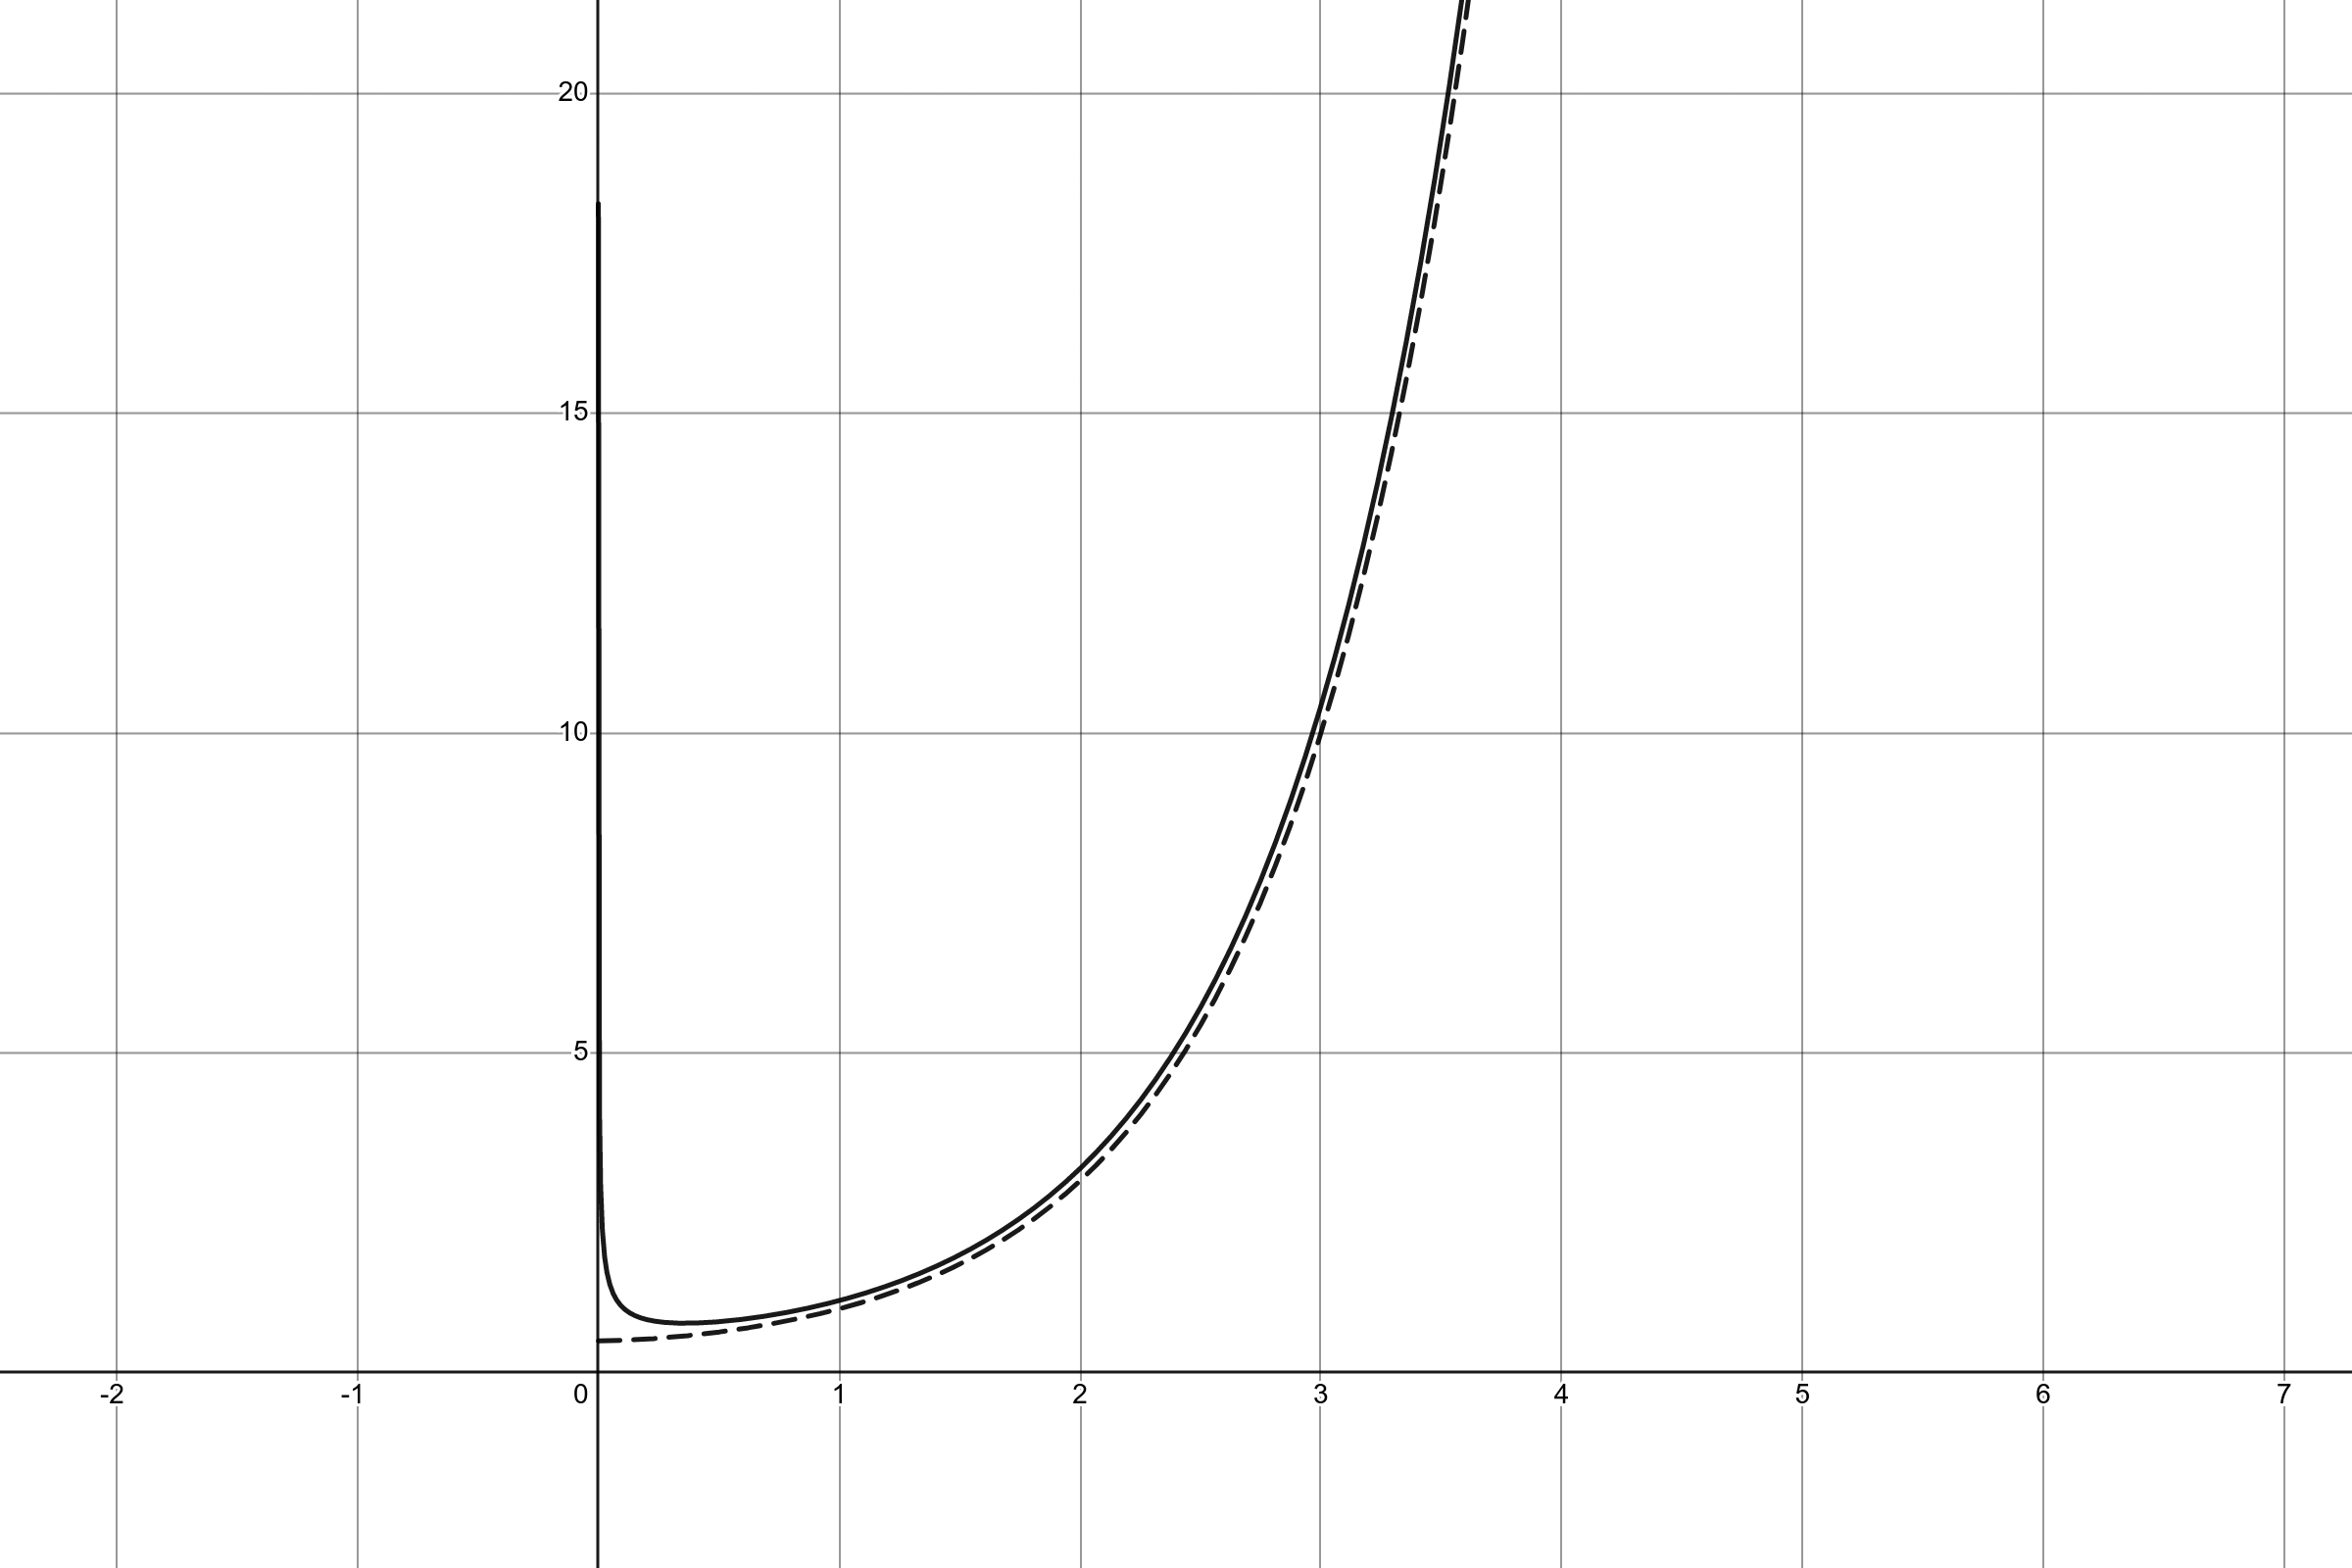
\includegraphics[width=\textwidth]{desmos-graph.png}
        \caption{La linea continua è il grafico di \eqref{stirling} mentre quella tratteggiata è il grafico di \eqref{orig}}
    \end{figure}
\end{homeworkProblem}

\end{document}
